%-----------------------------------------------------------------------------------------------------------------------------------------------%
%	The MIT License (MIT)
%	Copyright (c) 2015 Jan Küster
%-----------------------------------------------------------------------------------------------------------------------------------------------%

%============================================================================%
%	DOCUMENT DEFINITION
%============================================================================%

%we use article class because we want to fully customize the page and dont use a cv template
\documentclass[10pt,A4]{article}	


%----------------------------------------------------------------------------------------
%	ENCODING
%----------------------------------------------------------------------------------------

%we use utf8 since we want to build from any machine
\usepackage[utf8]{inputenc}		

%----------------------------------------------------------------------------------------
%	LOGIC
%----------------------------------------------------------------------------------------

% provides \isempty test
\usepackage{xifthen}

%----------------------------------------------------------------------------------------
%	FONT
%----------------------------------------------------------------------------------------

% some tex-live fonts - choose your own

%\usepackage[defaultsans]{droidsans}
%\usepackage[default]{comfortaa}
%\usepackage{cmbright}
\usepackage[default]{raleway}
%\usepackage{fetamont}
%\usepackage[default]{gillius}
%\usepackage[light,math]{iwona}
%\usepackage[thin]{roboto} 

% set font default
\renewcommand*\familydefault{\sfdefault} 	
\usepackage[T1]{fontenc}

% more font size definitions
\usepackage{moresize}		


%----------------------------------------------------------------------------------------
%	PAGE LAYOUT  DEFINITIONS
%----------------------------------------------------------------------------------------

%debug page outer frames
%\usepackage{showframe}			


%define page styles using geometry
\usepackage[a4paper]{geometry}		

% for example, change the margins to 2 inches all round
\geometry{top=1.75cm, bottom=-.6cm, left=1.5cm, right=1.5cm} 	

%use customized header
\usepackage{fancyhdr}				
\pagestyle{fancy}

%less space between header and content
\setlength{\headheight}{-5pt}		


% %customize entries left, center and right
% \lhead{}
% \chead{ \small{Jan Küster  $\cdot$ Consultant and Software Engineer $\cdot$  Bremen, Germany  $\cdot$  \textcolor{sectcol}{\textbf{info@jankuester.com}}  $\cdot$ +49 176 *** *** **}}
% \rhead{}


%indentation is zero
\setlength{\parindent}{0mm}

%----------------------------------------------------------------------------------------
%	TABLE /ARRAY DEFINITIONS
%---------------------------------------------------------------------------------------- 

%for table layout
\usepackage{multicol}			
\usepackage{multirow}

%extended aligning of tabular cells
\usepackage{array}

\newcolumntype{x}[1]{%
>{\raggedleft\hspace{0pt}}p{#1}}%


%----------------------------------------------------------------------------------------
%	GRAPHICS DEFINITIONS
%---------------------------------------------------------------------------------------- 

%for header image
\usepackage{graphicx}

%for floating figures
\usepackage{wrapfig}
\usepackage{float}
%\floatstyle{boxed} 
%\restylefloat{figure}

%for drawing graphics		
\usepackage{tikz}				
\usetikzlibrary{shapes, backgrounds,mindmap, trees}


%----------------------------------------------------------------------------------------
%	Color DEFINITIONS
%---------------------------------------------------------------------------------------- 

\usepackage{color}

%accent color
\definecolor{sectcol}{RGB}{255,150,0}

%dark background color
\definecolor{bgcol}{RGB}{110,110,110}

%light background / accent color
\definecolor{softcol}{RGB}{225,225,225}


%============================================================================%
%	DEFINITIONS
%============================================================================%

%----------------------------------------------------------------------------------------
% 	HEADER
%----------------------------------------------------------------------------------------

% remove top header line
\renewcommand{\headrulewidth}{0pt} 

%remove botttom header line
\renewcommand{\footrulewidth}{0pt}	  	

%remove pagenum
\renewcommand{\thepage}{}	

%remove section num		
\renewcommand{\thesection}{}			

%----------------------------------------------------------------------------------------
% 	ARROW GRAPHICS in Tikz
%----------------------------------------------------------------------------------------

% a six pointed arrow pointing to the left
\newcommand{\tzlarrow}{(0,0) -- (0.2,0) -- (0.3,0.2) -- (0.2,0.4) -- (0,0.4) -- (0.1,0.2) -- cycle;}	

% include the left arrow into a tikz picture
% param1: fill color
%
\newcommand{\larrow}[1]{
	\begin{tikzpicture}[scale=0.58]
		\filldraw[fill=#1!100,draw=#1!100!black] \tzlarrow
	\end{tikzpicture}
}

%----------------------------------------------------------------------------------------
%	custom sections
%----------------------------------------------------------------------------------------

% create a coloured box with arrow and title as cv section headline
% param 1: section title
%
\newcommand{\cvsection}[1]{
	% \vspace{8pt}
	\colorbox{sectcol}{
	\mystrut \makebox[1\linewidth][l]{
		\textcolor{white}{\textbf{#1}}\hspace{4pt}
		}
		}
	% \vspace{8pt}
}

%create a coloured arrow with title as cv meta section section
% param 1: meta section title
%
\newcommand{\metasection}[2]
{
\begin{tabular*}{1\textwidth}{p{2.4cm} p{11cm}}
\larrow{bgcol}	\normalsize{\textcolor{sectcol}{#1}}&#2\\[12pt]
\end{tabular*}
}

%----------------------------------------------------------------------------------------
%	 CV EVENT
%----------------------------------------------------------------------------------------

% creates a stretched box as cv entry headline followed by two paragraphs about 
% the work you did
% param 1:	event time i.e. 2014 or 2011-2014 etc.
% param 2:	event name (what did you do?)
% param 3:	institution (where did you work / study)
% param 4:	what was your position
% param 5:	some words about your contributions
%
\newcommand{\cvevent}[5]
{
\vspace{8pt}

\begin{tabular*}{1\textwidth}{p{3.3cm}  p{9.8cm} x{3.9cm}}
	\textcolor{bgcol}{#1} 	& \textbf{#2} \\ 
	 						& \textcolor{sectcol}{#3} \\
\end{tabular*}

\textcolor{softcol}{\hrule}

\vspace{6pt}
\begin{tabular*}{1\textwidth}{p{3.3cm} p{13.4cm}}
	&	\textcolor{bgcol}{--}  #4\\[3pt]
	&	\textcolor{bgcol}{--}  #5\\[6pt]
\end{tabular*}
}

% creates a stretched box as cv skill
\newcommand{\cvskill}[7]
{
\vspace{8pt}
\begin{tabular*}{1\textwidth}{p{3.3cm} p{13.4cm}}
	\textbf{#1} 		&	\textcolor{bgcol}{$\bullet$ }  #2\\[3pt]
						&	\textcolor{bgcol}{$\bullet$ }  #3\\[3pt]
						&	\textcolor{bgcol}{$\bullet$ }  #4\\[3pt]
						&	\textcolor{bgcol}{$\bullet$ }  #5\\[6pt]
						&	\textcolor{bgcol}{$\bullet$ }  #6\\[6pt]
						&	\textcolor{bgcol}{$\bullet$ }  #7\\[6pt]
\end{tabular*}
\textcolor{softcol}{\hrule}
}

% creates a stretched box as 
\newcommand{\cveventmeta}[2]
{
	\mbox{\mystrut \hspace{87pt}\textit{#1}}\\
	#2
}

%----------------------------------------------------------------------------------------
% CUSTOM STRUT FOR EMPTY BOXES
%----------------------------------------- -----------------------------------------------
\newcommand{\mystrut}{\rule[-.3\baselineskip]{0pt}{\baselineskip}}

%----------------------------------------------------------------------------------------
% CUSTOM LOREM IPSUM
%----------------------------------------------------------------------------------------
\newcommand{\lorem}
{Lorem ipsum dolor sit amet, consectetur adipiscing elit. Donec a diam lectus.}


%============================================================================%
%	DOCUMENT CONTENT
%============================================================================%
\begin{document}


%use our custom fancy header definitions
\pagestyle{fancy}	


%---------------------------------------------------------------------------------------
%	TITLE HEADLINE
%----------------------------------------------------------------------------------------
\vspace{-20.55pt}

% use this for multiple words like working titles etc.
%\hspace{-0.25\linewidth}\colorbox{bgcol}{\makebox[1.5\linewidth][c]{\hspace{46pt}\HUGE{\textcolor{white}{\textsc{Jan Küster}} } \textcolor{sectcol}{\rule[-1mm]{1mm}{0.9cm}} \parbox[b]{5cm}{   \large{ \textcolor{white}{{IT Consultant}}}\\
% \large{ \textcolor{white}{{Resume}}}}
%}}

% use this for single words, e.g. CV or RESUME etc.
\hspace{-0.25\linewidth}\colorbox{bgcol}{\makebox[1.5\linewidth][c]{\HUGE{\textcolor{white}{\textsc{Jan Küster}} } \textcolor{sectcol}{\rule[-1mm]{1mm}{0.9cm}} \HUGE{\textcolor{white}{\textsc{Resume}} } }}


%----------------------------------------------------------------------------------------
%	HEADER IMAGE
%----------------------------------------------------------------------------------------

\begin{figure}[H]
\begin{flushright}
	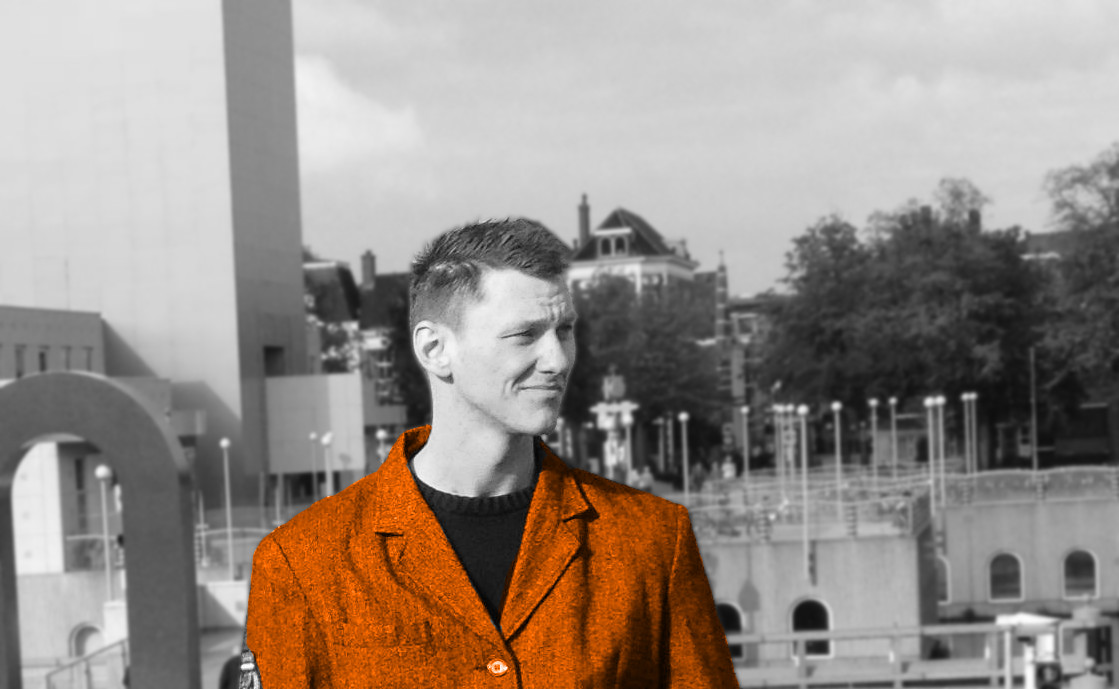
\includegraphics[trim= 320 130 460 210,clip,width=0.2\linewidth]{myfoto.jpg}	%trimming relative to image size!
\end{flushright}
\end{figure}

%----------------------------------------------------------------------------------------
%	META SECTION
%----------------------------------------------------------------------------------------

\vspace{-114pt}

\metasection{Status:}{M.Sc. Digital Media, Fullstack JS Engineer}
\metasection{Fields:}{Project Management, Software Development, Consulting} 
\metasection{Tech:}{Meteor, Javascript, Bootstrap, Mongodb, Git, Webstorm, Sourcetree}
\metasection{Loves:}{Global Game Jam, Sci-Fi series, Stackoverflow, Fitness and Martial Arts}

\vspace{6pt}

%----------------------------------------------------------------------------------------
%	SUMMARY (optional)
%----------------------------------------------------------------------------------------

\cvsection{Summary}\\
I am a digital media graduate (M.Sc.) with project experience in educational research as well as in 
the private sector. During my studies I focused on e-assessment software and moved over to b2b 
software for IBM Notes Domino.

Currently I develop and evaluate the next generation learning management system with Meteor based 
on an extensive nursing curriculum for healthcare education.  I also love fitness, martial arts, 
video games, news and Sci-Fi series.\\[-2pt]

%============================================================================%
%	CV SECTIONS AND EVENTS (MAIN CONTENT)
%============================================================================%

%---------------------------------------------------------------------------------------
%	EXPERIENCE
%----------------------------------------------------------------------------------------
\cvsection{Experience}

\cvevent{09/2021 - Present}{Fullstack Javascript Engineer}{University of Bremen}
{Invent a realtime classroom management using Meteor and React}
{Design software architecture and leading development}

\cvevent{02/2021 - 07/2021}{IT Consultant for IBM XPages and Notes Domino}{We4IT GmbH Bremen}
{Realize projects in XPages and We4IT Aveedo, monitor project status, conduct reports}
{Integrated Camunda BPMN engine and BPMN.IO modeler in We4IT Aveedo}

\cvevent{04/2020 - 12/2020}{Scientific Employee / Software Development}{University of Bremen}
{Invented a flexible assessment framework, targeting industrial trainees}
{Supervised software development lifecycle, Recruited team members}

\cvevent{08/2019 - Present}{Project Management Simulation Training}{Getoq Consulting}
{Performed a two-day project simulation from management perspective}{Topics included customer contracts, change management, controlling, operational tasks}


%---------------------------------------------------------------------------------------
%	EDUCATION SECTION
%--------------------------------------------------------------------------------------
\cvsection{Education}

\cvevent{2015 / 07}{Graduated as M.Sc. Digital Media}{University of Bremen}
{Master Thesis: Semi Automated Scoring in Technology Based Assessment}
{Developed and evaluated an algorithm for semi automated scoring of spreadsheet data}

\cvevent{2012 - 2013}{Master Project - PrIMA}{University of Bremen}
{Co-Invented a touch table application for medical support, co-developed software (Java) }
{Formed a scrum team, maintained project dev server (Debian), surveyed target audience}

\cvevent{2012 - 2015}{Master Studies Digital Media}{University of Bremen}
{Inter-cultural classes in English, covering special topics in computer science and design}
{Professionalized in research methods, software development and e-assessment}

\cvevent{2009 - 2010}{Semester Abroad}{University of Melbourne}
{Mastered six months of study and trans-cultural experience in Melbourne, Australia}
{Finished machine programming, information visualization, professional essay writing}

%---------------------------------------------------------------------------------------
%	SKILLS SECTION
%--------------------------------------------------------------------------------------
\cvsection{Skills}

\cvskill{Software}
{Python}
{C, C++}
{Git, Gitflow}
{Docker, containerized development}
{Embedded development (Arduino, ESP32)}
{Docker, containerized development}

\cvskill{Software}
{Python}
{C, C++}
{Git, Gitflow}
{Docker, containerized development}
{Embedded development (Arduino, ESP32)}
{Docker, containerized development}

%-------------------------------------------------------------------------------------------------
%	ARTIFICIAL FOOTER (fancy footer cannot exceed linewidth) 
%--------------------------------------------------------------------------------------------------

\null
\vspace*{\fill}
% \hspace{-0.25\linewidth}\colorbox{bgcol}{\makebox[1.5\linewidth][c]{\mystrut \small \textcolor{white}{www.jankuester.com} $\cdot$ \textcolor{white}{github.com/jankapunkt}}}

%============================================================================%
%	DOCUMENT END
%============================================================================%
\end{document}
